\documentclass[11pt]{scrartcl}
 \usepackage{tkz-graph} 
 \begin{document} 
 \begin{center} 
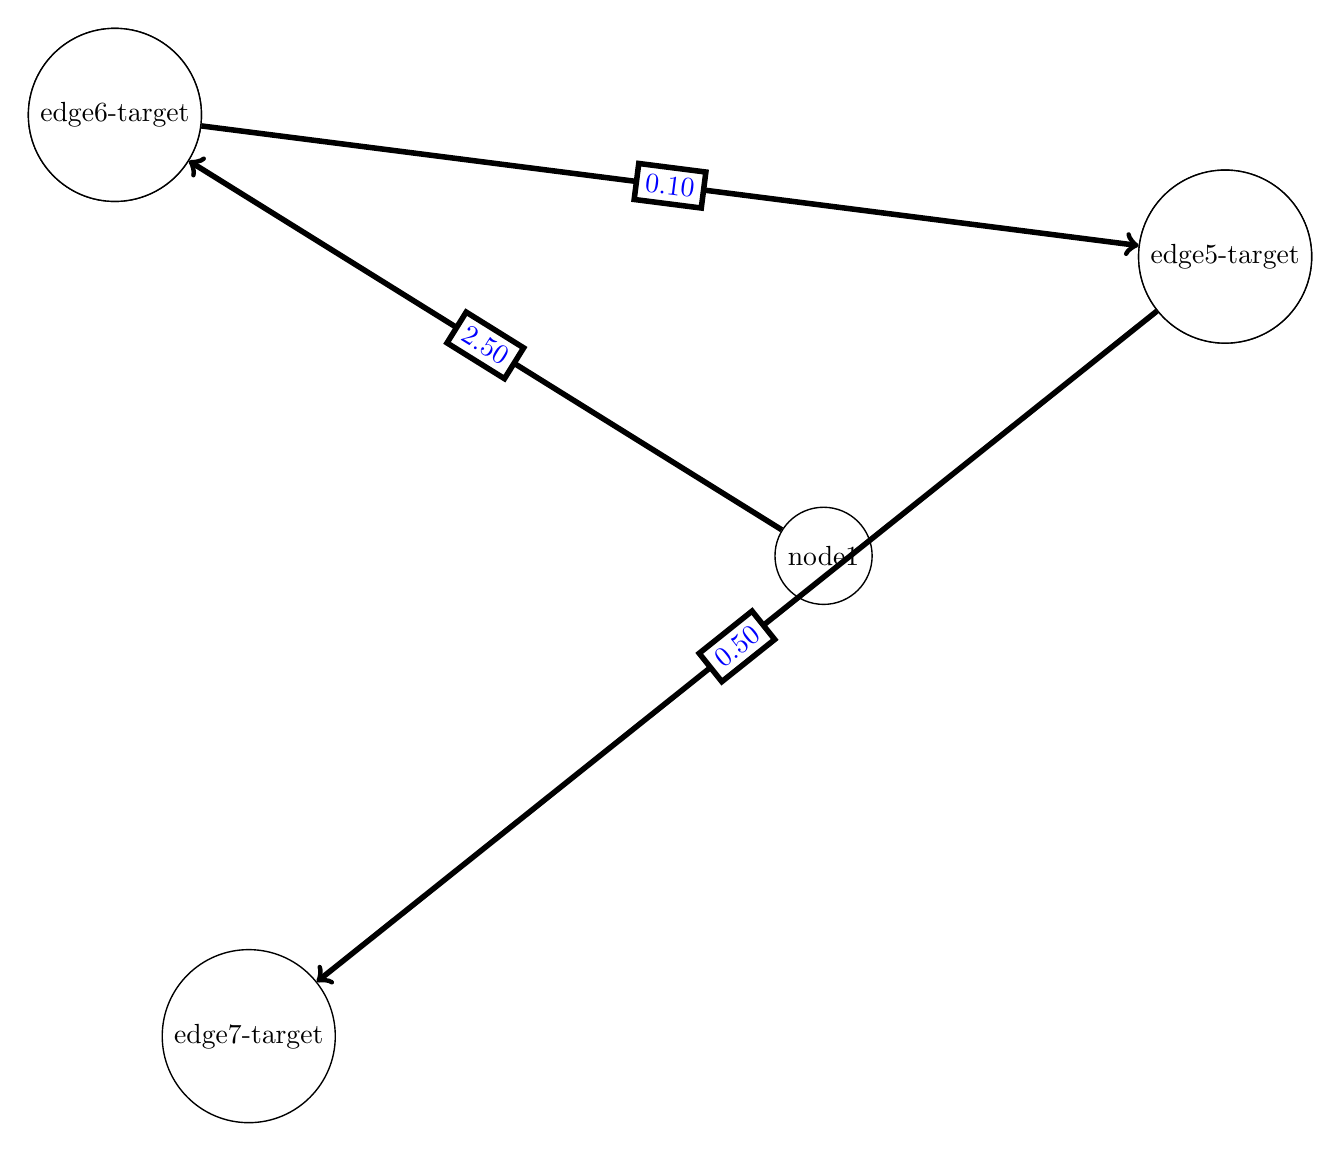
\begin{tikzpicture}  
 \SetVertexNormal[Shape      = circle, FillColor  = orange, LineWidth  = 2pt]
\SetUpEdge[lw  = 2pt,  color      = black,  labelcolor = white,  labeltext  = red, labelstyle = {sloped,draw,text=blue}]
\GraphInit[vstyle=Normal] 
   \SetGraphUnit{10} 
\tikzset{VertexStyle/.append  style={fill}}
\Vertex[x=9.2 ,y=10.5]{node1}
\tikzset{VertexStyle/.append  style={fill}}
\Vertex[x=0.2 ,y=16.1]{edge6-target}
\tikzset{EdgeStyle/.style={->}}
\Edge[label=$2.50$](node1)(edge6-target)
\tikzset{VertexStyle/.append  style={fill}}
\Vertex[x=0.2 ,y=16.1]{edge6-target}
\tikzset{VertexStyle/.append  style={fill}}
\Vertex[x=14.3 ,y=14.3]{edge5-target}
\tikzset{EdgeStyle/.style={->}}
\Edge[label=$0.10$](edge6-target)(edge5-target)
\tikzset{VertexStyle/.append  style={fill}}
\Vertex[x=14.3 ,y=14.3]{edge5-target}
\tikzset{VertexStyle/.append  style={fill}}
\Vertex[x=1.9 ,y=4.4]{edge7-target}
\tikzset{EdgeStyle/.style={->}}
\Edge[label=$0.50$](edge5-target)(edge7-target)
\end{tikzpicture}
\mbox{Total weight: 12435}

 \end{center}  
 \end{document}
